\documentclass[a4paper, 12pt, reqno]{amsart}

\newcommand{\titl}{Actuarial Mathematics Homework 13}

\usepackage{amssymb}
\usepackage{amsfonts}
\usepackage[margin=1in]{geometry}
\usepackage[english]{babel}
\usepackage[colorlinks, pdftitle={\titl},
    pdfauthor={Moritz M. Konarski}]{hyperref}
\usepackage{enumitem}
\setlist[enumerate]{label = (\alph*)}
\usepackage{graphicx}
\usepackage{float}
\renewcommand{\baselinestretch}{1.25}
\usepackage{actuarialsymbol}

\title{\titl}
\author{Moritz M. Konarski}
\date{\today}

\begin{document}

\maketitle

\section*{Parmenter Exercises 5}

\subsection*{5--1} 

Find a price to yield 8\% convertible semiannually for a 10--year, 1,000 face
value bond that has 9\% convertible semiannually.
\begin{equation}\nonumber
    \begin{gathered}
        P = (Fr)\ax{\angln i} + C v^n   \\
        P = (1,000 \cdot 0.045)\ax{\angl{20} 0.04} + 1,000 v^{20}   \\
        P = 45\ax{\angl{20} 0.04} + 1,000 v^{20}   \\
        P = 1,067.95163
    \end{gathered}
\end{equation}

\subsection*{5--2} 

1,000 par value bond, $r=0.055$, semiannually at Jan. 1 and Jul. 1. Redeemed on
Jul. 1, 2001. Bond is bought Jan. 1 1999. Find a price so it yields 12\%
semiannually.
\begin{equation}\nonumber
    \begin{gathered}
        P = (1,000 \cdot 0.055)\ax{\angl{5} i} + 1000 \cdot v^5 \\
        P = 55 \cdot \ax{\angl{5} 0.06} + 1000 \cdot v^5 \\
        P = 978.93818
    \end{gathered}
\end{equation}

\subsection*{5--5} 

\begin{equation}\nonumber
    \begin{gathered}
        P_1 = 879.58 = 50 \ax{\angln} + 1000 v^n        \\
        v^n = \frac{879.58 - \frac{50}{i}}{1000 - \frac{50}{i}}     \\
        n = \frac{\log \left( \frac{879.58 - \frac{50}{i}}{1000 - \frac{50}{i}}
            \right)}{\log v}
        n = 22      \\
        P_2 = 70 \ax{\angl{22}} + 1000 v^{22}
        P_2 = 1120.41582
    \end{gathered}
\end{equation}

\subsection*{5--6} 

\begin{equation}\nonumber
    \begin{gathered}
        P = 9 \ax{\angl{20}} + 110 v^{20}     \\
        A_1 = 8 \ax{\angl{20}} + 100 v^{20}     \\
        A_2 = 10 \ax{\angl{20}} + 100 v^{20}     \\
        P = A_1 + 0.1 A_2       \\
        P = 8 \ax{\angl{20}} + 100 v^{20} + 0.1 (10 \ax{\angl{20}} + 100 v^{20})\\
        P = 9 \ax{\angl{20}} + 110 v^{20}     \\
    \end{gathered}
\end{equation}

\subsection*{5--8}

Using the iterative method, we can find $i$ using
\begin{equation}\nonumber
    \begin{gathered}
        i = \frac{Fr(1-v^n)}{P-Cv^n}           \\
        i = 0.03293
    \end{gathered}
\end{equation}
per half year

\subsection*{5--9}

Using the iterative method for $i$, and $r = i + 0.01$, we use the iterative
method to find $i$
\begin{equation}\nonumber
    \begin{gathered}
        i = \frac{Fr(1-v^n)}{P-Cv^n}           \\
        i = 0.07266
    \end{gathered}
\end{equation}

\subsection*{5--10}

We start with a 6\% annual coupon, for 5 years, with a yield of 4\%. A new bond
has a 5\% coupon rate, how long does it have to run to have the same yield
rate.
\begin{equation}\nonumber
    \begin{gathered}
        P = \ax{\angl{5}} Fr + F v^5        \\
        F = 1                               \\
        P = \ax{\angl{5}} \cdot 0.06 + v^5           \\
        P = 0.05 \ax{\angln} + v^n          \\
        P = 0.05 \frac{1 - v^n}{i} + v^n          \\
        \ax{\angl{5}} r + v^5 = \frac{0.05}{i} - \frac{0.05v^n}{i} + v^n    \\
        v^n = \frac{0.06\ax{\angl{5}} + v^5 - \frac{0.05}{i}}{1
            - \frac{0.05}{i}}   \\
        n = 11.22578
    \end{gathered}
\end{equation}

\subsection*{5--11}

\begin{equation}\nonumber
    \begin{gathered}
        P = Fr\ax{\angln} + C v^n           \\
        n = \frac{\ln \left( \frac{P - \frac{Fr}{i}}{C 
            - \frac{Fr}{i}}\right)}{\ln v}  \\
        n = 9                               \\
        2n = 18                             \\
        P = 100 \cdot 0.05 \cdot \ax{\angl{18}0.075} + 100 \cdot v^{18}    \\
        P = 76.82317
    \end{gathered}
\end{equation}

\subsection*{5--13}

\begin{enumerate}
    \item just after the 7th coupon has been paid
        \begin{equation}\nonumber
            \begin{gathered}
                B_7 = 45 \ax{\angl{13}} + 1000 v^{13} \\
                B_7 = 1049.92824
            \end{gathered}
        \end{equation}
    \item 4 months after the 7th coupon has been paid
        \begin{equation}\nonumber
            \begin{gathered}
                X = B_7 (1 + \frac{2}{3}i) = 1077.92633
            \end{gathered}
        \end{equation}
    \item just before the 8th coupon is paid
        \begin{equation}\nonumber
            \begin{gathered}
                X = B_7 (1 + i) = 1091.92537
            \end{gathered}
        \end{equation}
\end{enumerate}

\subsection*{5--14}

$P = 978.93818$
\begin{enumerate}
    \item June 30, 1999, 11:59 pm
        \begin{equation}\nonumber
            \begin{gathered}
                P(1+i) = 1037.67447
            \end{gathered}
        \end{equation}
    \item Jul 1, 2000 12:01 am
        \begin{equation}\nonumber
            \begin{gathered}
                P(1+i) - Fr = 982.67447
            \end{gathered}
        \end{equation}
    \item March 1, 2001 - value on Jan 1, 2001 plus a bit
        \begin{equation}\nonumber
            \begin{gathered}
                X = B_5 \cdot (1 + \frac{2}{6}i) = 1015.18868
            \end{gathered}
        \end{equation}
    \item March 1, 2001 - value on Jan 1, 2001 plus a bit
        \begin{equation}\nonumber
            \begin{gathered}
                X = B_5 \cdot (1 + \frac{23}{24}i) = 1052.51180
            \end{gathered}
        \end{equation}
\end{enumerate}

\subsection*{5--16}

A screenshot of my program.
\begin{figure}[H]
    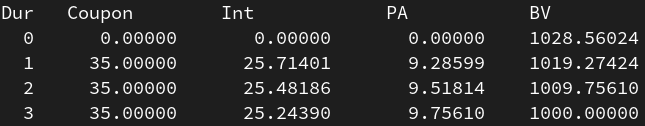
\includegraphics[width=0.7\textwidth]{../graphics/5-16}
    \caption{5--16}
\end{figure}

\subsection*{5--17}

A screenshot of my program.
\begin{figure}[H]
    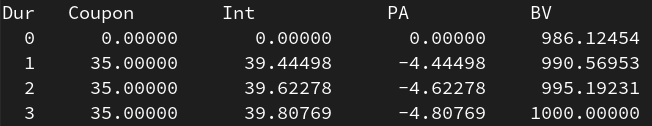
\includegraphics[width=0.7\textwidth]{../graphics/5-17}
    \caption{5--17}
\end{figure}

\subsection*{5--18}

A screenshot of my program.
\begin{figure}[H]
    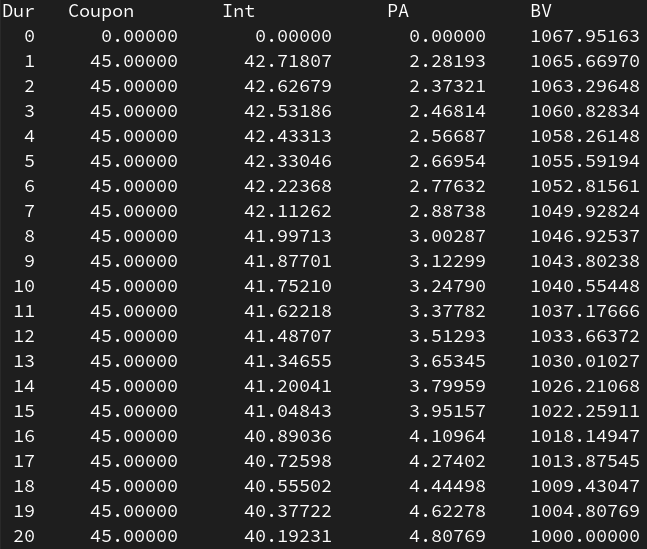
\includegraphics[width=0.7\textwidth]{../graphics/5-18}
    \caption{5--18}
\end{figure}

\subsection*{5--19}

Code for the program is available upon request. The above questions are solved
using this program.

\subsection*{5--20}

\begin{equation}\nonumber
    \begin{gathered}
        B_{n-1} = Fr \ax{\angl{1}} + C v^1  \\
        F = C       \\
        B_{n-1} = F(r \ax{\angl{1}} + v^1)  \\
        B_{n-1} = 5000(0.03 \ax{\angl{1}} + v^1)  \\
        B_{n-1} = 5024.39024
    \end{gathered}
\end{equation}

\subsection*{5--21}

\begin{equation}\nonumber
    \begin{gathered}
        B_{n-1} = Fr \ax{\angl{n-1}} + C v^{n-1}  \\
        \frac{B_{n-1}}{F} = \frac{r}{i} - \frac{rv^{n-1}}{i} + v^{n-1}      \\
        v^{n-1} = \frac{B_{n-1}}{F} - \frac{r}{i}       \\
        n = \frac{\ln \left( \frac{B_{n-1}}{F} - \frac{r}{i} \right)}{\ln v}+1\\
        n = 2                               \\
        P = 45 \ax{\angl{2}} + 1000 v^2     \\
        P = 972.49911                       \\
        D = F - P = 27.5                    \\
    \end{gathered}
\end{equation}

\subsection*{5--22}

\begin{equation}\nonumber
    \begin{gathered}
        \sum_{j=1}^{20} B_j \cdot i = 910.03968
    \end{gathered}
\end{equation}

\subsection*{5--23}

Principal adjustment is $PA$
\begin{equation}\nonumber
    \begin{gathered}
        PA_{18} = 36            \\
        PA_{18} = Fr - B_{t-1} i            \\
        36 = Fr - i ((Fr)\ax{\angl{40-17}} - C v^{40-17})            \\
        r = \frac{36 + i C v^{23}}{F(1 - \ax{\angl{23}})}           \\
        r = 0.07375                                         \\
        PA_{29} = Fr - B_{t-1} \\
        PA_{29} = 737.5 - i (737.5 \ax{\angl{12}} - C v^{12})\\
        PA_{29} = 68.33875
    \end{gathered}
\end{equation}

\subsection*{5--24}

\begin{enumerate}
    \item 12\% per year $\rightarrow$ $i = \sqrt{1.12} - 1 = 0.0583$
        \begin{equation}\nonumber
            \begin{gathered}
                P = 1000 r \ax{\angl{20}} + C v^{20} \\
                P = 903.46609
            \end{gathered}
        \end{equation}
    \item 1\% per month $\rightarrow$ $i = 1.01^6 - 1 = 0.06152$
        \begin{equation}\nonumber
            \begin{gathered}
                P = 1000 r \ax{\angl{20}} + C v^{20} \\
                P = 869.48008
            \end{gathered}
        \end{equation}
\end{enumerate}

\subsection*{5--25}

\begin{equation}\nonumber
    \begin{gathered}
        \bar d = \frac{\sum_{j=1}^{20}j v^j 50 + 50 v^{20}1000}
            {\sum_{j=1}^{20}v^j 50 + 50 v^{20}1000}             \\
        \bar d = 22.10101
    \end{gathered}
\end{equation}

\subsection*{5--26}

1000 face par value, 10 year bond, $r=0.03$ for 5, then $r=0.035$ for the last
5. Find the price if the following yield is anticipated
\begin{enumerate}
    \item earn 7\% as half year
        \begin{equation}\nonumber
            \begin{gathered}
                P = P_1 + v^{10} P_2        \\
                P = 1102.44089
            \end{gathered}
        \end{equation}
    \item earn 14\% per year, $i = \sqrt{1.14} - 1$
        \begin{equation}\nonumber
            \begin{gathered}
                P = P_1 + v^{10} P_2        \\
                P = 1131.10854
            \end{gathered}
        \end{equation}
\end{enumerate}

\subsection*{5--27}

10 year bond, 1000 par value, coupon starts at 200, decreases by 20 each time,
until it reaches 20.
\begin{enumerate}
    \item find $P$ for $i = 0.12$
        \begin{equation}\nonumber
            \begin{gathered}
                P = (Da)_{\angl{10}} + 1000 v^{10}
                P = 1046.93607
            \end{gathered}
        \end{equation}
    \item find the yield rate if the bond is purchased at face value, solved
        through iteration
        \begin{equation}\nonumber
            \begin{gathered}
                i = \frac{(10 - \ax{\angl{20}}) 20}{P - 1000v^{10}}
                i = 0.12963
            \end{gathered}
        \end{equation}
\end{enumerate}

\subsection*{5--28}

1000 bond, 15 year bond, 60 per coupon, callable for the last 10 dates. Find
the price to guarantee a yield rate of:
\begin{enumerate}
    \item 7\%, the yield rate is higher than the coupon rate, we should
        consider the last value
        \begin{equation}\nonumber
            \begin{gathered}
                P = 1000 \cdot \ax{\angl{30}} + 1000 v^{30}     \\
                P = 875.90959
            \end{gathered}
        \end{equation}
    \item 5\%, the yield rate is smaller than the coupon rate, we consider the
        first value
        \begin{equation}\nonumber
            \begin{gathered}
                P = 1000 \cdot \ax{\angl{20}} + 1000 v^{20}     \\
                P = 1124.62210
            \end{gathered}
        \end{equation}
    \item 6\%, in this case the redemption date does not matter. Because the
        coupon rate and the yield rate are the same, for a price of 1000,
        regardless of redemption date, the bond will yield 6\%.
\end{enumerate}

\end{document}
